\documentclass{beamer}
\usetheme{Berlin}
\usepackage[swedish]{babel}
\usepackage[utf8]{inputenc}
\usepackage{textpos}
\usepackage{xcolor}
\usepackage{listings}


\definecolor{wingblue}{HTML}{C9E2D9}
\definecolor{bodyblue}{HTML}{84B1A1}
\definecolor{stomacheblue}{HTML}{395355}
\definecolor{lightbrown}{HTML}{D7A274}
\definecolor{darkbrown}{HTML}{B97232}
\definecolor{codegreen}{rgb}{0,0.6,0}
\definecolor{codegray}{rgb}{0.5,0.5,0.5}
\definecolor{codepurple}{rgb}{0.58,0,0.82}
\definecolor{backcolour}{rgb}{0.95,0.95,0.92}

\lstset{
	language=Python,
    %backgroundcolor=\color{backcolour},   
    commentstyle=\color{codegreen},
    keywordstyle=\color{magenta},
    numberstyle=\tiny\color{codegray},
    stringstyle=\color{codepurple},
    basicstyle=\footnotesize,
    breakatwhitespace=false,         
    breaklines=true,                 
    captionpos=b,                    
    keepspaces=true,                 
    numbers=left,                    
    numbersep=5pt,                  
    showspaces=false,                
    showstringspaces=false,
    showtabs=false,                  
    tabsize=4
}

\setbeamercolor{alerted text}{fg=orange}
\setbeamercolor{background canvas}{bg=white}
\setbeamercolor{block body alerted}{bg=normal text.bg!90!black}
\setbeamercolor{block body}{bg=normal text.bg!90!black}
\setbeamercolor{block body example}{bg=normal text.bg!90!black}
\setbeamercolor{block title alerted}{use={normal text,alerted text},fg=alerted text.fg!75!normal text.fg,bg=normal text.bg!75!black}
\setbeamercolor{block title}{bg=blue}
\setbeamercolor{block title example}{use={normal text,example text},fg=example text.fg!75!normal text.fg,bg=normal text.bg!75!black}
\setbeamercolor{fine separation line}{}
\setbeamercolor{frametitle}{fg=black}
\setbeamercolor{item projected}{fg=black}
\setbeamercolor{normal text}{bg=bodyblue,fg=black}
\setbeamercolor{palette sidebar primary}{use=normal text,fg=normal text.fg}
\setbeamercolor{palette sidebar quaternary}{use=structure,fg=structure.fg}
\setbeamercolor{palette sidebar secondary}{use=structure,fg=structure.fg}
\setbeamercolor{palette sidebar tertiary}{use=normal text,fg=normal text.fg}
\setbeamercolor{section in sidebar}{fg=brown}
\setbeamercolor{section in sidebar shaded}{fg=grey}
\setbeamercolor{separation line}{}
\setbeamercolor{sidebar}{bg=red}
\setbeamercolor{sidebar}{parent=palette primary}
\setbeamercolor{structure}{bg=black, fg=wingblue}
\setbeamercolor{subsection in sidebar}{fg=bodyblue}
\setbeamercolor{subsection in sidebar shaded}{fg=stomacheblue}
\setbeamercolor{title}{fg=black}
\setbeamercolor{titlelike}{fg=brown}

\author[Mattias Salo]{
\includegraphics[width=1.7cm]{../logo.png}\\Mattias Salo}
\title{Python vs. Scratch}
\institute{CoderDojo Linköping}

\begin{document}

\begin{frame}
\maketitle
\end{frame}

\addtobeamertemplate{frametitle}{}{%
\begin{textblock*}{100mm}(-0.96cm,0.72\textheight)

\includegraphics[width=1.4cm]{../logo.png}
\end{textblock*}}

\begin{frame}[fragile]
	\frametitle{Vad är skillanden?}

	\begin{itemize}
		\item{Scratch använder klossar}
		\item{Python använder text}
	\end{itemize}
	\begin{columns}[c] % the "c" option specifies center vertical alignment
    \column{.5\textwidth} % column designated by a command
    \begin{center}
     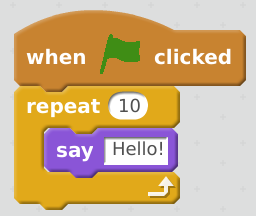
\includegraphics[width=0.7\textwidth]{blocks/for_10.png}
     \end{center}
    \column{.5\textwidth}
\begin{lstlisting}[language=Python]
for i in range(10):
    print("Hello!")
\end{lstlisting}
    \end{columns}
\end{frame}

\begin{frame}
	\frametitle{Hur ser Python ut?}
	Python används framför allt med en såkallad kommandotolk. (t.ex. DOS/BASH)
	(På Windows: klicka på start och sök efter cmd.exe, MAC: Spotlight-sök efter terminal)\\
	\begin{center}
	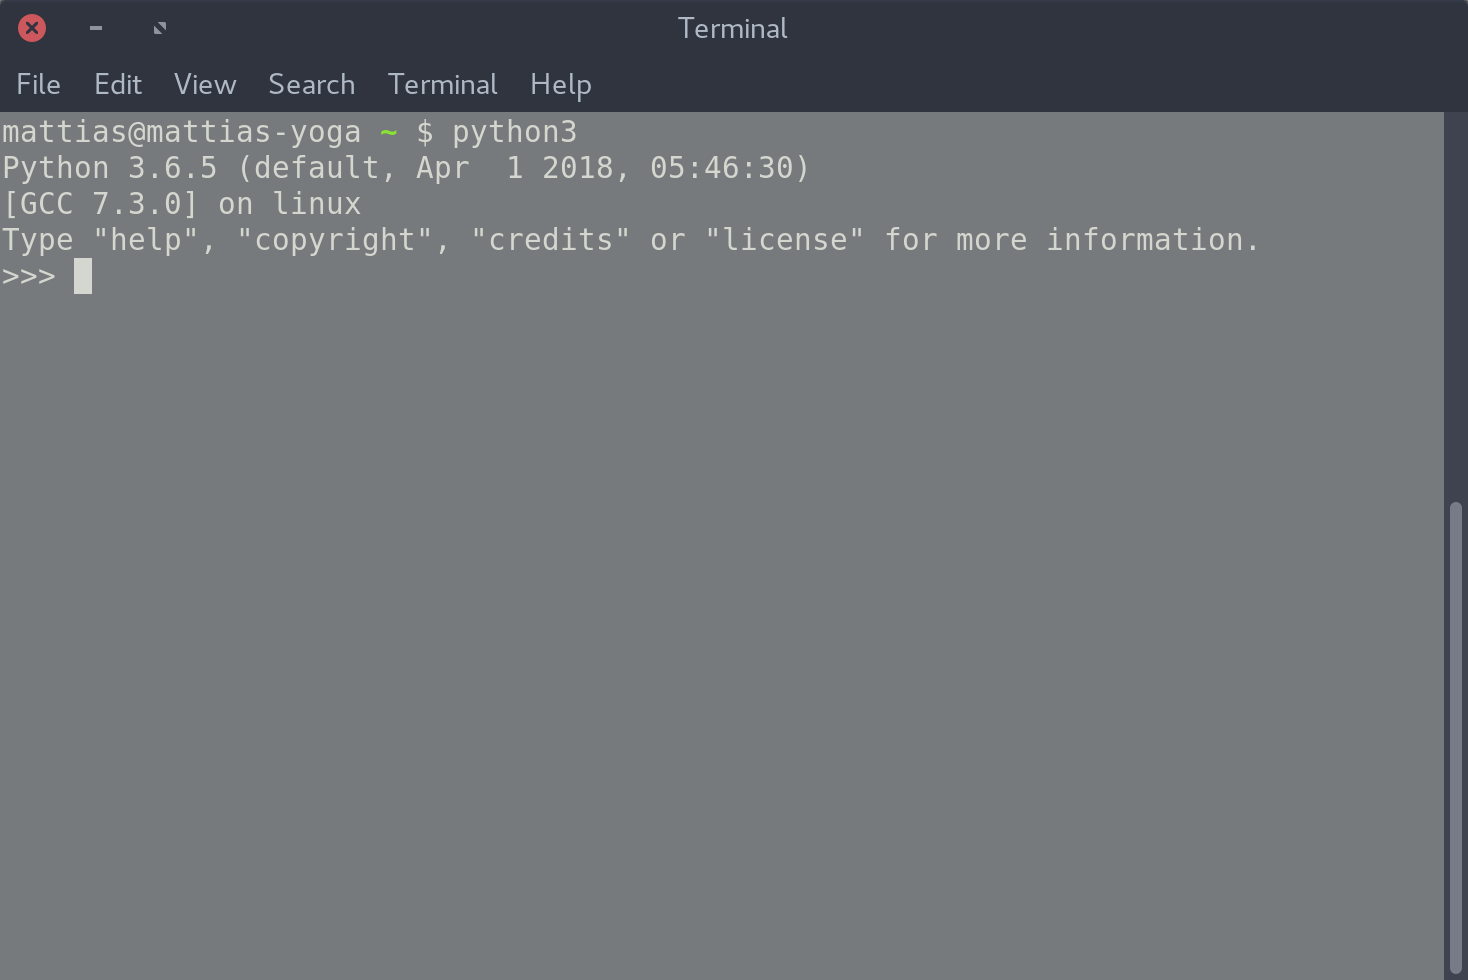
\includegraphics[width=0.9\textwidth]{other_pics/python_terminal_ex.png}
	\end{center}
\end{frame}

\begin{frame}[fragile]
	\frametitle{loopar}

	\begin{columns}[c] % the "c" option specifies center vertical alignment
    	\column{.5\textwidth} % column designated by a command
    	\begin{center}
     		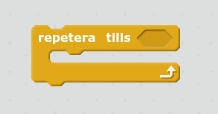
\includegraphics[width=0.45\textwidth]{blocks/while.png}
     	\end{center}
     	\begin{center}
     	     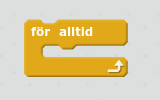
\includegraphics[width=0.45\textwidth]{blocks/while_true.png}
     	\end{center}
     	\begin{center}
     	     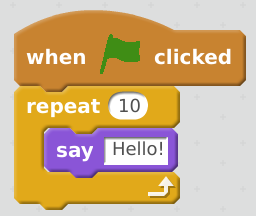
\includegraphics[width=0.45\textwidth]{blocks/for_10.png}
     	\end{center}

    	\column{.5\textwidth}
		\begin{lstlisting}[language=Python]
			while():
    			#code
		\end{lstlisting}
		\
		
		\begin{lstlisting}[language=Python]
			while(True):
		    	#code
		\end{lstlisting}
		\
		
		\begin{lstlisting}[language=Python]
			for i in range(10):
			    print("Hello!")
		\end{lstlisting}
    \end{columns}
\end{frame}


\end{document}